\newpage
\begin{figure}[hbt!]
\chapter{環境設定}
\section{碰撞檢測}
\end{figure}
1.可探測(Detectable),可讓感測器感測到物體。在本遊戲中,球應該將Detectable打開,這樣才可以感測到進球,而bubbleRob機器人則要把Detectable關掉,不然機器人碰到感測器也會得分。\
\begin{center}
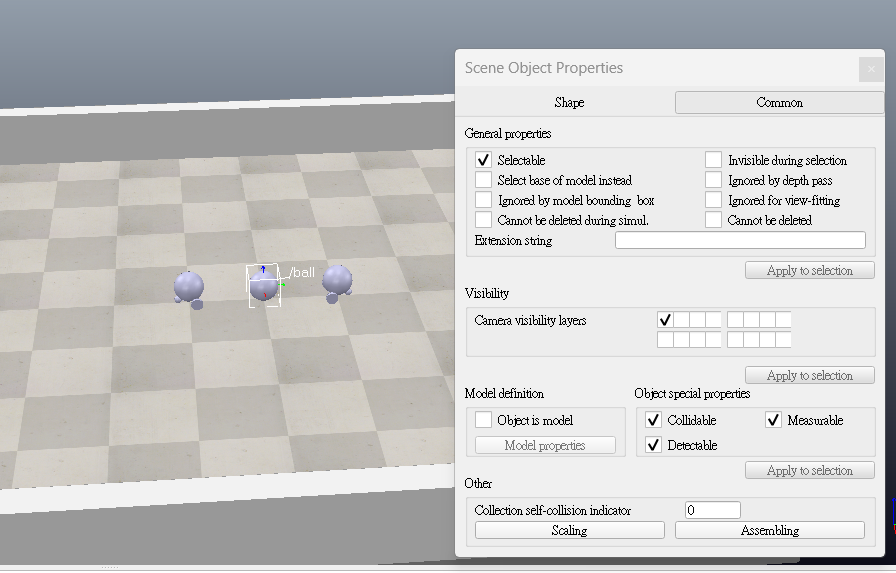
\includegraphics[angle=0,width=12cm]{48.1}\\
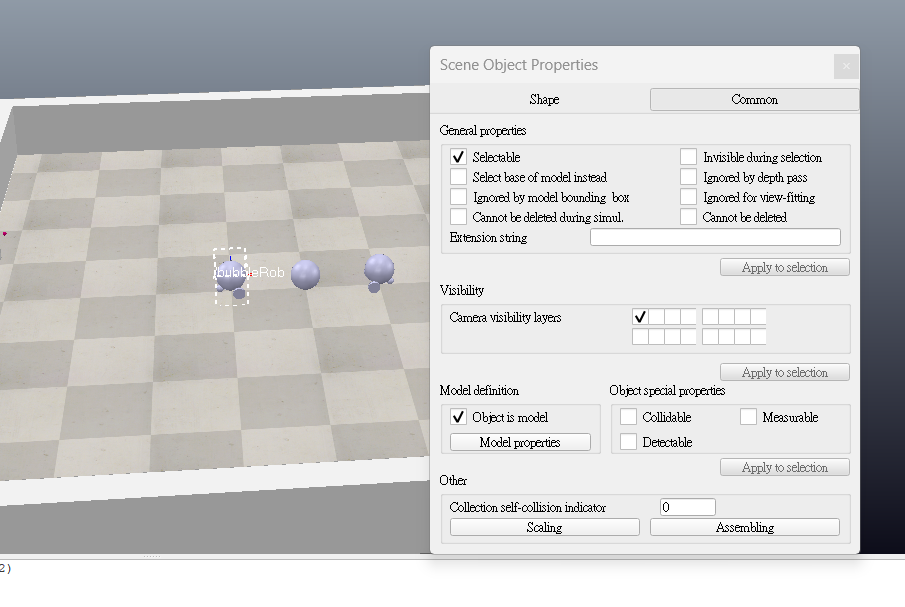
\includegraphics[angle=0,width=12cm]{48.2}
\end{center}
\newpage
2.在球框前加入射線感測器(Ray type),這樣球進框就一定會碰到感測器,射線感測器不能貼地不然感測不到。
\begin{center}
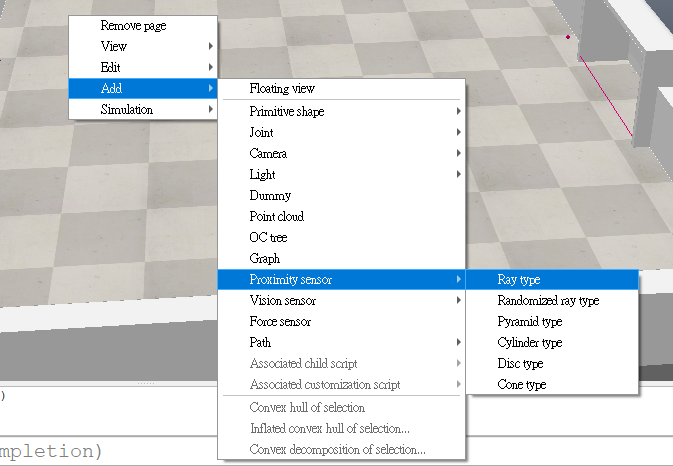
\includegraphics[angle=0,width=10cm]{48.5}
\end{center}

3.球框及圍牆的Body is respondable要打開不然球會穿過去,而Body is dynamic則要關上不然球框會亂動。
\begin{center}
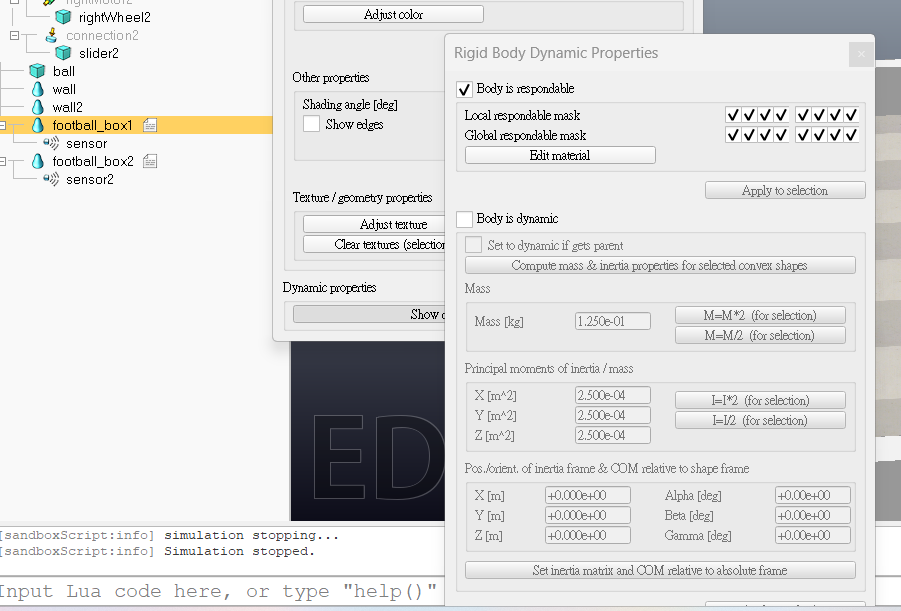
\includegraphics[angle=0,width=10cm]{48.3}
\end{center}

4.開啟Connectivity->Visualization,從http://127.0.0.1:23020/ 中可看見。
\begin{center}
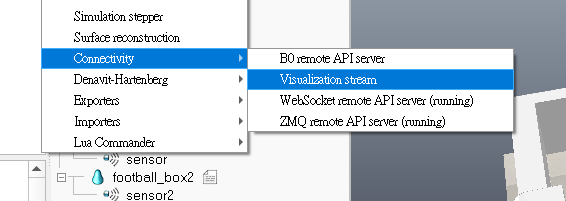
\includegraphics[angle=0,width=10cm]{4810}
\end{center}